\section{วิธีการเร็กกิวลาร์ไลซ์เซชัน}

\hspace{1cm} ในโครงงานวิจัยเรื่องนี้ จะพบปัญหา Ill-posed ซึ่งทำให้การแก้ปัญหานั้นเกิดความยากลำบากขึ้น จึงจำเป็นต้องหาวิธีแก้ปัญหา Ill-posed ให้เป็นปัญหา Well-posed ก่อนนำไปแก้ปัญหาถัดไป

\subsection{ปัญหา Well-posed และปัญหา Ill-posed}

\begin{Definition}
    (ปัญหา Well-posed) จะเรียกปัญหาต่อไปนี้ว่าเป็นปัญหา Well-posed เมื่อปัญหามีคุณสมบัติดังนี้
    \begin{enumerate}
        \item มีคำตอบ
        \item มีเพียงคำตอบเดียว
        \item คำตอบขึ้นอยู่กับความต่อเนื่อง
    \end{enumerate}    
    หากปัญหาไม่ตรงคุณสมบัติใดจากทั้ง 3 ข้อ จะเรียกปัญหาดังกล่าวว่า ปัญหา Ill-posed
\end{Definition}

\subsection{ปัญหาย้อนกลับ}
\hspace{1cm}ปัญหาย้อนกลับ (Inverse problem) คือปัญหาสำหรับการกู้คืนข้อมูลพารามิเตอร์จากตัวแบบทางคณิตศาสตร์โดยใช้ข้อมูลบางพารามิเตอร์ที่ทราบค่าอยู่ ซึ่งโดยทั่วไปแล้วปัญหาย้อนกลับนี้มักจะเป็นปัญหา Ill-posed

\begin{Example}
    \hspace{1cm} สำหรับตัวอย่างปัญหาย้อนกลับ เช่น จงหาค่า $x$ และ $y$ ที่ทำให้ $x+y = 5$ จะเห็นว่ามีชุดของคำตอบ $x+y=5$ อยู่มากมาย ซึ่งทำให้เป็นปัญหา Ill-posed เนื่องจากคำตอบของปัญหาไม่ได้มีเพียงชุดเดียว
    \label{example:x_plus_y_5}
\end{Example}

\hspace{1cm} ในส่วนของการต่อเติมภาพที่เสียหายนั้นเป็นปัญหาย้อนกลับและเป็นปัญหา Ill-posed ด้วยเนื่องจากคำตอบในบริเวณที่จะต่อเติมไม่ได้มีเพียงคำตอบเดียว ตัวอย่างเช่น ภาพที่ \ref{image:meme_elephant} ภาพช้างทีเสียหาย\footnote{ภาพจาก https://9gag.com/gag/aer4VwB สืบค้นเมื่อ 10 มีนาคม 2562} ในบริเวณภาพสีแดงซึ่งภาพเกิดความเสียหายขึ้น อาจจะมีคำตอบเป็นขาของช้าง หรือมีคำตอบเป็นสิงโตดังในภาพก็ได้

\begin{figure}[H]
    \centering
    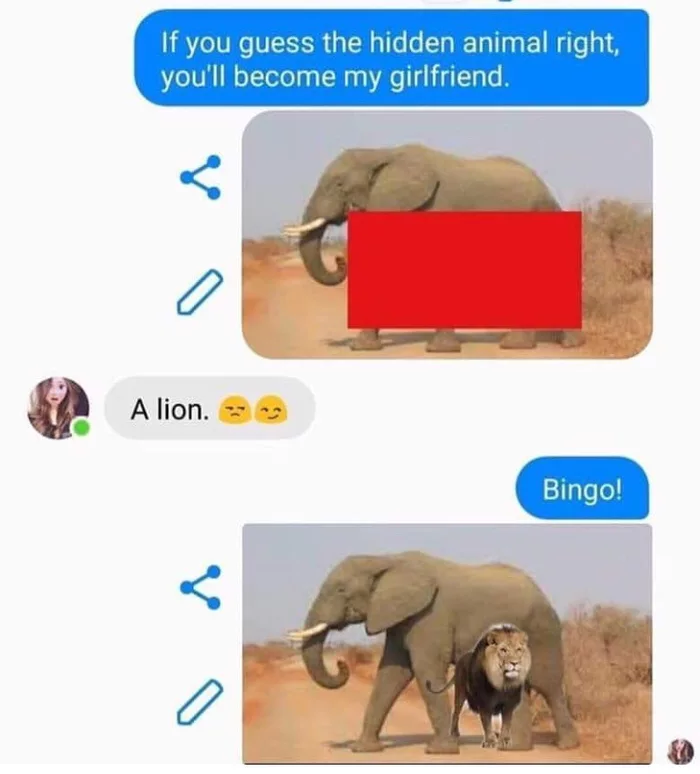
\includegraphics[width=0.35\linewidth]{image/meme_elephant.png}
    \caption[a]{ตัวอย่างการต่อเติมภาพที่ไม่มีคำตอบเฉพาะเจาะจง}
    \label{image:meme_elephant}
\end{figure}

\begin{Example}
    ตัวอย่างปัญหาย้อนกลับ เมื่อ $z$ เป็นภาพซึ่ง นิยามอยู่ใน $ \Omega \in \mathbb{R}^2$ $\eta$ คือสัญญาณรบกวนแบบเกาส์เซียนที่มีส่วนเบี่ยงเบนมาตราฐานเป็น $\sigma^2$ และ $u$ คือภาพที่มีสัญญาณรบกวน โดยที่ $u = z + \eta$ เราสามารถนำสัญญาณรบกวนออกได้โดยหา $u$ ที่เหมาะสมจาก
    \begin{align}
        \underset{min}{u} \Big\{ \Bigl| \int_{\Omega} |u-z|^2 d\Omega - \sigma^2 \Bigr| \Big\}
    \end{align}    
    ซึ่ง $u$ ที่เหมาะสมมีหลายคำตอบจึงได้ว่า $u$ นี่เป็นปัญหา Ill-posed
    \label{equation:denosing_model}
\end{Example}


\subsection{เร็กกิวลาไลซ์เซชัน}
\hspace{1cm} วิธีเร็กกิวลาไลซ์เซชัน (Regularization) เป็นวิธีการทำให้ปัญหาย้อนกลับกลายเป็นปัญหา Well-posed ได้ โดยคุณ Tikhonov และคุณ Arsenin \cite{ref:regularization} ได้นำเสนอวิธีการสำหรับจัดการปัญหาค่าเหมาะสมโดยใช้การแนะนำวิธีการแก้ปัญหานี้โดยการทำให้ปัญหามีคำตอบอยู่ในชุดของคำตอบใด คำตอบหนึ่ง หรือทำให้มีคุณลักษณะที่เฉพาะเจาะจง

\hspace{1cm} จากตัวอย่าง \ref{example:x_plus_y_5} สามารถทำให้คำตอบเจาะจงขึ้นได้ โดยการเพิ่มเงื่อนไขเข้าไปว่า $x+y=5$ เมื่อ $\sqrt{x^2+y^2}$ มีค่าน้อยที่สุด

\hspace{1cm} จากตัวอย่าง \ref{equation:denosing_model} เราสามารทำให้คำตอบเจาะจงขึ้นได้โดยการเพิ่มพจน์เข้าไปดังนี้

\begin{align}
    \underset{min}{u} \Big\{ \Bigl| \int_{\Omega} |u-z|^2 d\Omega - \sigma^2 \Bigr| + \alpha \int_{\Omega} |\nabla u|^2 \Big\}
    \label{equation:denosing_reglarization_model}
\end{align}

\hspace{1cm} โดยจะเรียกพจน์แรกว่าพจน์ปรับค่าข้อมูล (Data fitting term) และพจน์ที่ 2 ว่าพจน์เร็กกิวลาไลซ์เซชัน (Regularization term) โดยเมื่อคำตอบ $u$ มีค่าเกรเดียนต์ที่น้อยแล้วจะได้ผลลัพธ์ออกมาเป็นภาพที่ไม่มีสัญญาณรบกวน